\section{Background}\label{sec:background}
We briefly explain the concept of edit distance and its relation to the longest common subsequence. We then present the sequential algorithm from Myers, which was the basis for our parallel implementation.

% Give a short, self-contained summary of necessary
% background information. For example, assume you present an
% implementation of sorting algorithms. You could organize into sorting
% definition, algorithms considered, and asymptotic runtime statements. The goal of the
% background section is to make the paper self-contained for an audience
% as large as possible. As in every section
% you start with a very brief overview of the section. Here it could be as follows: In this section 
% we formally define the sorting problem we consider and introduce the algorithms we use
% including a cost analysis.

% Explain the algorithm you use including their costs.
% As an aside, don't talk about "the complexity of the algorithm.'' It's incorrect, problems have a complexity, not algorithms.

% \mypar{Longest common subsequence}
% The longest common subsequence problem is the problem of finding the longest sequence that two input sequences have in common. A related problem is finding the longest common substring. However, in that case the solution sequence needs to appear consecutively within the input string.

\mypar{Edit distance}
The edit distance refers to the minimum number of changes required to transform one string into another. In the case where we only consider insertions and deletions, and exclude substitutions, the LCS problem is equivalent to finding the edit distance. All symbols that do not appear in the LCS count towards the edit distance.

To transform the first string into the second, we perform deletions for all symbols in the first sequence that are not part of the LCS and similarly insertions for the second sequence. Those changes are referred to as an edit script. % and the total number of changes is the edit distance.

%\mypar{Diff program} 
%In the context of computer science, it is a common problem to compare source files to different versions. In order to visualize changes better, a diff program can display the minimal number of changes by highlighting all symbols that are part of the edit script.

\mypar{Myers' algorithm}
Myers \cite{myers_anond_1986} takes a greedy approach to finding the solution in the edit graph of two sequences. It has an asymptotic runtime of $O(nd)$ where $n$ is the total length of the two sequences and $d$ is the size of the minimum edit script. This algorithm performs well when the sequences are similar and have a small $d$.

For constructing the edit graph, shown in figure \ref{edit_graph}, the two sequences A and B are placed along a grid. The solution for the shortest edit script can be constructed by finding the shortest path from $(0,0)$ to the bottom right corner. A horizontal or vertical segment represents an edit. A diagonal can only be taken if the two input sequences are identical.

\begin{figure}[hbt]\centering
  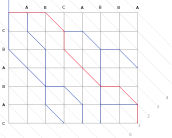
\includegraphics[width=0.9\linewidth]{images/edit-graph.pdf}
  \caption{Edit graph for comparison of two sequences \cite{edit_graph}. The solution for the shortest edit script is shown in red.
}
  \label{edit_graph}
\end{figure}

% Myers' algorithm pseudocode
\begin{algorithm}
\caption{Myers' LCS algorithm \cite{myers_anond_1986}}
\label{myers_algorithm}
\SetAlgoNoLine
\SetAlgoNoEnd
\DontPrintSemicolon
\scriptsize       % decrease font size

\KwSty{Constant} $MAX \in [0, M+N]$\;
$V:\ \KwSty{Integer}[-MAX\ ..\ MAX]$\;
\;
$V[1]\leftarrow 0$\;
\For{$d\leftarrow 0$ \KwTo $MAX$}{
    \For{$k\leftarrow -d$ \KwTo d in steps of 2}{
        \eIf{$k=-d$ or $k\ne d$ and $V[k-1]<V[k+1]$}{
            $x\leftarrow V[k+1]$\;
        }{
            $x\leftarrow V[k-1]+1$\;
        }
        $y\leftarrow x-k$\;
        \While{$x < N$ and $y < M$ and $a_{x+1} = b_{y+1}$}{$(x,y)\leftarrow (x+1,y+1)$\;}
        $V[k]\leftarrow x$\;
        \If{$x\ge N$ and $y \ge M$}{
            Length of shortest edit script is d\;
            \KwSty{STOP}\;
        }
    }
 }
\end{algorithm}

Myers' algorithm, shown in algorithm \ref{myers_algorithm}, goes through the diagonals shown in figure \ref{edit_graph} with an increasing edit distance and stores the coordinates of the furthest reachable point on each diagonal. The variables $N$ and $M$ represent the lengths of the sequences A and B.\\
To compute an entry on the diagonal $k$ and distance $d$, the previous paths can connect to it either by a horizontal or vertical move from its neighbors on the diagonals $k \pm 1$. Out of those two entries from the table for a distance of $d-1$, it takes the one with the higher x-value and follows the diagonal as long as the two sequences are identical. The new coordinates are then stored in the DP table.

The solution has been found once an entry reaches the coordinates $(N,M)$. The edit distance $d$ for that entry directly tells us the minimum edit distance. But the actual edit script has to be computed recursively.

\begin{figure}[hbt]\centering
  \includegraphics[width=0.95\linewidth]{images/dp_table.pdf}
  \caption{The DP table represents the furthest points on each diagonal that can be reached for a given edit distance. The arrows denote the dependencies of a single entry. The solution is marked in red and has an edit distance of 5.}
  \label{dp_table}
\end{figure}

Every entry depends on at most two entries from the previous row in the DP table (marked as arrows in figure \ref{dp_table}). If we only want the LCS length, it is not required to store the entire table, but only the previous row for the distance $d-1$. Thus the memory consumption is linear and no longer the limiting factor for very large input sequences. Myers presents an approach (``linear refinement'') to compute the solution recursively \cite{myers_anond_1986}. However, we will not go further into detail because it lies outside the scope of this report.
% Additionally, it is not necessary to store both coordinates. If we only store the x-coordinate for an entry, we can compute the intersection with the diagonal $k$ as $y = x - k$.
